\section{Subclasses, Superclasses, and Inheritance}

The EER model adds the following concepts:\\

\begin{itemize}
    \item \textbf{subclass} and \textbf{superclass}
    \item \textbf{specialization} and \textbf{generalization}
    \item \textbf{category} or \textbf{union type} (used to represent a collection of entities = union of objects of different entity types)
    \item \textbf{attribute and relationship inheritance}
\end{itemize}

A \textbf{subtype} or \textbf{subclass} of an entity type are used to represent subgroupings or subtypes of an entity that are meaningful. They need to be represented explicitly because of their significance to the database application. For example $EMPLOYEE$ can be distinguished in $SECRETARY$, $ENGINEER$ and $TECHNICIAN$.\\

The set in each of the subgroupings is a subset of the entities that belong to the $EMPLOYEE$ entity set. $EMPLOYEE$ is called the \textbf{superclass} or \textbf{supertype}. The relation between a superclass and a subclass is called \textbf{class/subclass relationship}. An entity can be a member of any number of subclasses. The EER notation is given on figure \ref{fig:subclasses}.\\

\begin{figure}[!h]
    \centering
    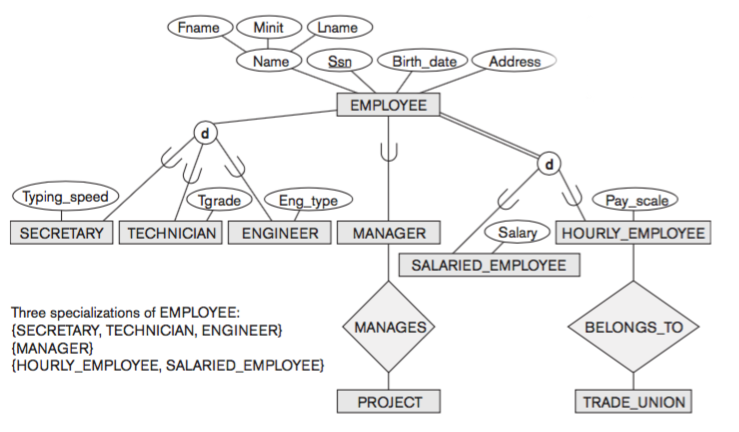
\includegraphics[scale=0.4]{chap4-1.png}
    \caption{EER notation to represent subclasses and specialization}
    \label{fig:subclasses}
\end{figure}

The \textbf{type} of an entity is defined by the attributes that it possesses and the relationship types in which it participates.\\

An entity that is a member of a subclass \textbf{inherits} all the attributes of the entity as a member of the superclass (= \textbf{type inheritance}). It also inherits all the relationships in which the superclass participates. A subclass can also have specific attributes and relationships.

\section{Specialization and generalization}

\subsection{Specialization}

\textbf{Specialization} is the process of defining a set of subclasses of an entity type. This set of subclasses is defined on the basis of some distinguishing characteristics of the entities in the superclass. There can be several specializations of the same entity type based based on different distinguishing characteristics.
Figure \ref{fig:subclasses} shows the EER representation. The subset symbols on each line indicate the direction of the superclass/subclass relationship.\\

An entity that belongs to a subclass represents the same real-world entity as the corresponding entity in the superclass.\\

There are two main reasons for including class/subclass relationships and specializations:\\

\begin{itemize}
    \item Certain attributes may apply to some but not all entities of the superclass entity type. A subclass is defined in order to group the entities to which these attributes apply.
    \item Some relationship types may be participated in only by entities that are members of the subclass. For example, only $HOURLY\_EMPLOYEE$ are related to the entity type $TRADE\_UNION$ by the relation $BELONGS\_TO$.
\end{itemize}
    
\subsection{Generalization}

\textbf{Generalization} is the process of suppressing the differences among several entity types (by identifying their common features) to generalize them into a \textbf{superclass}. The original entity types are special subclasses. For example $CAR$ and $TRUCK$ can be generalized in $VEHICLE$.

\section{Constraints and characteristics of specialization and generalization hierarchies}

\subsection{Constraints on Specialization and Generalization}

\textbf{Predicate-defined subclasses} are the ones for which we can determine the entities that will become members of each subclass by placing a condition on the value of some attribute of the superclass\\

\begin{figure}[!h]
    \centering
    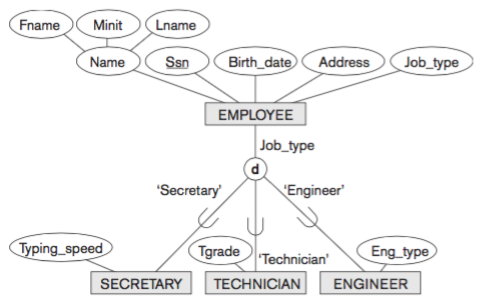
\includegraphics[scale=0.4]{chap4-2.png}
    \caption{Attribute-defined specialization on Job\_type}
    \label{fig:predicate}
\end{figure}

If all subclasses have their membership condition on the same attribute of the superclass, we call it an \textbf{attribute-defined} specialization and the attribute is called the \textbf{defining attribute} (cfr. figure \ref{fig:predicate}).\\

When there is no condition to determine membership in a subclass, it is called an \textbf{user-defined} subclass (membership determined by the user).\\

The \textbf{disjointness constraint} specifies that the subclasses of a specialization must be disjoint sets. An entity can be a member of at most one subclass. The representation is shown on figure \ref{fig:predicate} (the $d$ in the circle). Otherwise, the sets of entities may be \textbf{overlapping}. It is represented with a $o$ in a circle and not a $d$.\\

\textbf{A total (or completeness) specialization constraint} specifies that every entity in the superclass must be a member of at least one subclass in the specialization. It is represented by using a double line to connect the superclass to the circle (cfr. figure \ref{fig:subclasses}). A single line is used for \textbf{partial participation} which allows an entity not to belong to any subclass.\\

The \textbf{disjointness} and \textbf{completeness} constraints are independent.

\textbf{Rules for insertion and deletion}:\\

\begin{itemize}
    \item \textbf{Deleting} an entity from a superclass implies that it is automatically deleted from all the subclasses to which it belongs.
    \item \textbf{Inserting} an entity in a superclass implies that the entity is mandatorily inserted in all predicate-defined  subclasses for which the entity satisfies the defining predicate
    \item \textbf{Inserting} an entity in a superclass of a total specialization implies that the entity is mandatorily inserted in at least one of the subclasses
\end{itemize}

\subsection{Specialization and Generalization Hierarchies and Lattices}

A subclass may have further subclasses specified on it, forming a hierarchy or a lattice of specializations.\\

\begin{itemize}
    \item \textbf{Specialization hierarchy}: each subclass has only one parent (\textbf{tree} structure)
    \item \textbf{Specialization lattice}: a subclass can have several parents (cfr. figure \ref{fig:lattice})
\end{itemize}

In such a specialization lattice or hierarchy, a subclass inherits the attributes of all its predecessor superclasses.\\

\begin{figure}[!h]
    \centering
    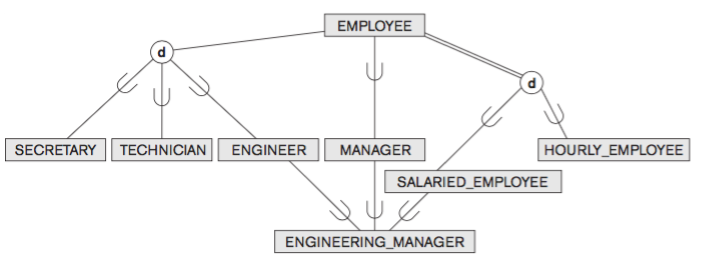
\includegraphics[scale=0.4]{chap4-3.png}
    \caption{A specialization lattice}
    \label{fig:lattice}
\end{figure}

A \textbf{shared subclass} is a subclass with more than one parent (\textbf{multiple inheritance}).\\

Some models and languages don't allow multiple inheritance and/or multiple types.

\subsection{Utilizing Specialization and Generalization in Refining Conceptual Schemas}

\textbf{Top-down conceptual refinement} is the process of starting with one entity type and then specializing it into several subclasses.

\textbf{Bottom-up conceptual synthesis} is the contrary. First start with the last level of subclassess and then generalize them. 

\section{Modeling of UNION Types Using Categories}

An \textbf{union type} or \textbf{category} is a subclass that represents a collection of entities from different entity types. For example if a vehicle can have three types of owner $PERSON$, $BANK$ or $COMPANY$, it is possible to create a category $OWNER$ that is a subclass of the union of the three entity sets (cfr. figure \ref{fig:category}). \\

\begin{figure}[!h]
    \centering
    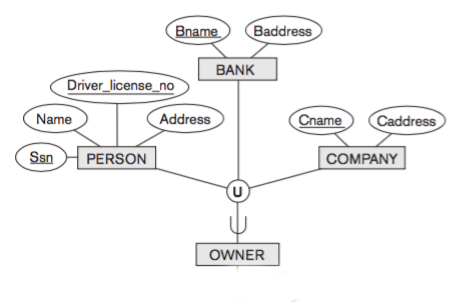
\includegraphics[scale=0.4]{chap4-4.png}
    \caption{Category OWNER}
    \label{fig:category}
\end{figure}

\textbf{Difference between a category and a shared subclass}:\\

\begin{itemize}
    \item \textbf{Category}: subset of the \textbf{union} of its superclasses. An entity belonging to a category must exist in only one of the superclasses. It inherits the attributes of the superclass to which it belongs.
    \item \textbf{Shared class}: subclass of each of the superclass. So an entity that is a member of a shared class must exists in all the superclasses' collections. Its entity set is a subset of the \textbf{intersection} of the entity sets. It inherits the attributes of all the superclasses
\end{itemize}

A \textbf{total} category holds the union of all the entities in its superclasses. It is represented with a double line connecting the category and the circle. A \textbf{partial} category holds a subset of the union.

\section{Design Choices and Formal Definitions}

\subsection{Design choices}

\textbf{Guidelines to guide the design process}:\\

\begin{itemize}
    \item Represent only those subclasses that are necessary to avoid extreme cluttering of the conceptual schema
    \item If a subclass has few specific (local) attributes and no specific relationships, it can be merged into the superclass (possibly add a type attribute).
    \item If all the subclasses of a specialization have few specific attributes and no specific relationships, they can be merged into the superclass and replaced with one or more type attributes
    \item Union types and categories should be avoided unless really necessary.
    \item The choice of disjoint/overlapping and total/partial depends on the miniworld being modeled.
\end{itemize}

\subsection{Formal Definitions for the EER Model Concepts}

\textbf{Definitions}:\\

\begin{itemize}
    \item \textbf{Class}: defines a type of entity and represents a set or collection of entities of that type.
    
    \item \textbf{Subclass}: class whose entities must always be a subset of the entities in another class called the \textbf{superclass}
    
    \item \textbf{Specialization}: set of subclasses Z=$\big\{$S1,S2,..,Sn$\big\}$ that have the same super class G called the \textbf{Generalized entity type} (or \textbf{superclass}). 
    
    The specialization is said to be \textbf{total} if $\bigcup_{i=1}^n S_i$ = G. 
    
    Z is \textbf{disjoint} if we have $S_i \bigcap S_j$ = $\emptyset$ for i$\neq$j. Otherwise it is \textbf{overlapping}
    
    \item \textbf{Predicate defined subclass}: if a predicate on the attributes is used to specify which entities are members of the subclass.
    
    Otherwise it is \textbf{user defined}
    
    \item \textbf{Attribute-defined specialization} : if a predicate A = $c_i$ (with A an attribute of the superclass and $c_i$ a constant from the domain of A) is used to specify membership in each subclass $S_i$.
    
    \item \textbf{Category}: class T that is a subset of the union of n defining superclass $D_1$ .. $D_n$. So we have T $\subseteq$ ($D_1$ $\cup$ .. $\cup$ $D_n$).
    
    A predicate $p_i$ on the attributes of $D_i$ can be used to specify the members of each $D_i$ that are members of T.
    
    T $\subseteq$ ($D_{1}[p_1]$ $\cup$ .. $\cup$ $D_{n}[p_n]$).
 \end{itemize}
 
 The definition of relationship type must be extended to allow any class to participate in a relationship (replace the word entity type by class in the definition).
 
 %\section{Data Abstraction, Knowledge Representation, and Ontology Concepts}
 
 %\textcolor{red}{\textbf{TODO}} But not really important I think ...